\documentclass[11pt, a4paper]{article}
\usepackage{graphicx}
\usepackage{amsmath}
\usepackage{listings}
\usepackage{color}
\usepackage{fancyhdr}
\usepackage[utf8]{inputenc}
\usepackage{gensymb}
\usepackage[%  
    colorlinks=true,
    pdfborder={0 0 0},
    linkcolor=red
]{hyperref}

\definecolor{dkgreen}{rgb}{0,0.6,0}
\definecolor{gray}{rgb}{0.5,0.5,0.5}
\definecolor{mauve}{rgb}{0.58,0,0.82}

\lstset{frame=tb,
  language=Python,
  aboveskip=3mm,
  belowskip=3mm,
  showstringspaces=false,
  columns=flexible,
  basicstyle={\small\ttfamily},
  numbers=none,
  numberstyle=\tiny\color{gray},
  keywordstyle=\color{blue},
  commentstyle=\color{dkgreen},
  stringstyle=\color{mauve},
  breaklines=true,
  breakatwhitespace=true,
  tabsize=3
}



\title{EE2703-Assignment6-2}
\author{EE19B094}
\date{April 2021}

\setlength{\headheight}{15pt}
\pagestyle{fancy}
\fancyhf{}
\rhead{Assignment - 6-2}
\lhead{EE2703 - Applied Programming Lab}
\rfoot{Page \thepage}

\begin{document}

\maketitle
\newpage
\begin{abstract}
    In this assignment, we will look at how to analyze and solve for LTI systems using standard libraries in python .We restrict our analysis to systems with rational polynomial transfer functions. More specifically we consider 3 systems: A forced oscillatory system, A coupled system of Differential Equations and an RLC low pass filter  
\end{abstract}

\section{Question 1,2}
We are given an equation describing forced oscillatory system(with 0 initial conditions) as:
\begin{equation}
    \ddot x + 2.25x = f(t)
\end{equation}
where x is the output and f(t) is the input.

Thus the transfer function of the system is 
\begin{equation}
   H(s) = \frac{1}{s^2+2.25}
\end{equation}
Now, we are given input f(t) as $cos(1.5t)e^{-0.5t}u_0(t)$ i.e.
\begin{equation}
   F(s) = \frac{s+0.5}{(s+0.5)^2+2.25}
\end{equation}
Thus the output will be X(s) = H(s)F(s)
\begin{equation}
   X(s) = \frac{s+0.5}{((s+0.5)^2+2.25)(s^2+2.25)}
\end{equation}
Now, we use the sp.lit() function to find the plot the time domain output x(t).
We also do the same for similar input function but with different decay constant

\begin{lstlisting}
#Q1
def Q_1(freq,decay_constant):
	#Function to get laplace equation for input for given values of frequency and decay constant
	def input_laplace(freq,decay_constant):
		num = np.poly1d([1,decay_constant])
		den = np.poly1d([1,2*decay_constant,decay_constant*decay_constant+freq*freq])
		return num,den

	#Input function
	input_num,input_den = input_laplace(freq,decay_constant)

	#Output function by multiplying transfer function and input function
	output_laplace_num = input_num
	output_laplace_den = np.polymul(input_den,[1,0,2.25])
	output_laplace = sp.lti(output_laplace_num,output_laplace_den)

	#Get time domain output for time = 0 to 5001
	time,output_time = sp.impulse(output_laplace,None,np.linspace(0,50,5001))

	#Plot graph
	g1 = General_Plotter("Time$\longrightarrow$","Position$\longrightarrow$","Q1: Decay = %s"%decay_constant,[])
	g1.line_plot(time,output_time)


Q_1(1.5,0.5)	#Decay constant = 0.5
Q_1(1.5,0.05)	#Decay constant = 0.05
\end{lstlisting}

\begin{figure}[tbh!]
\centering
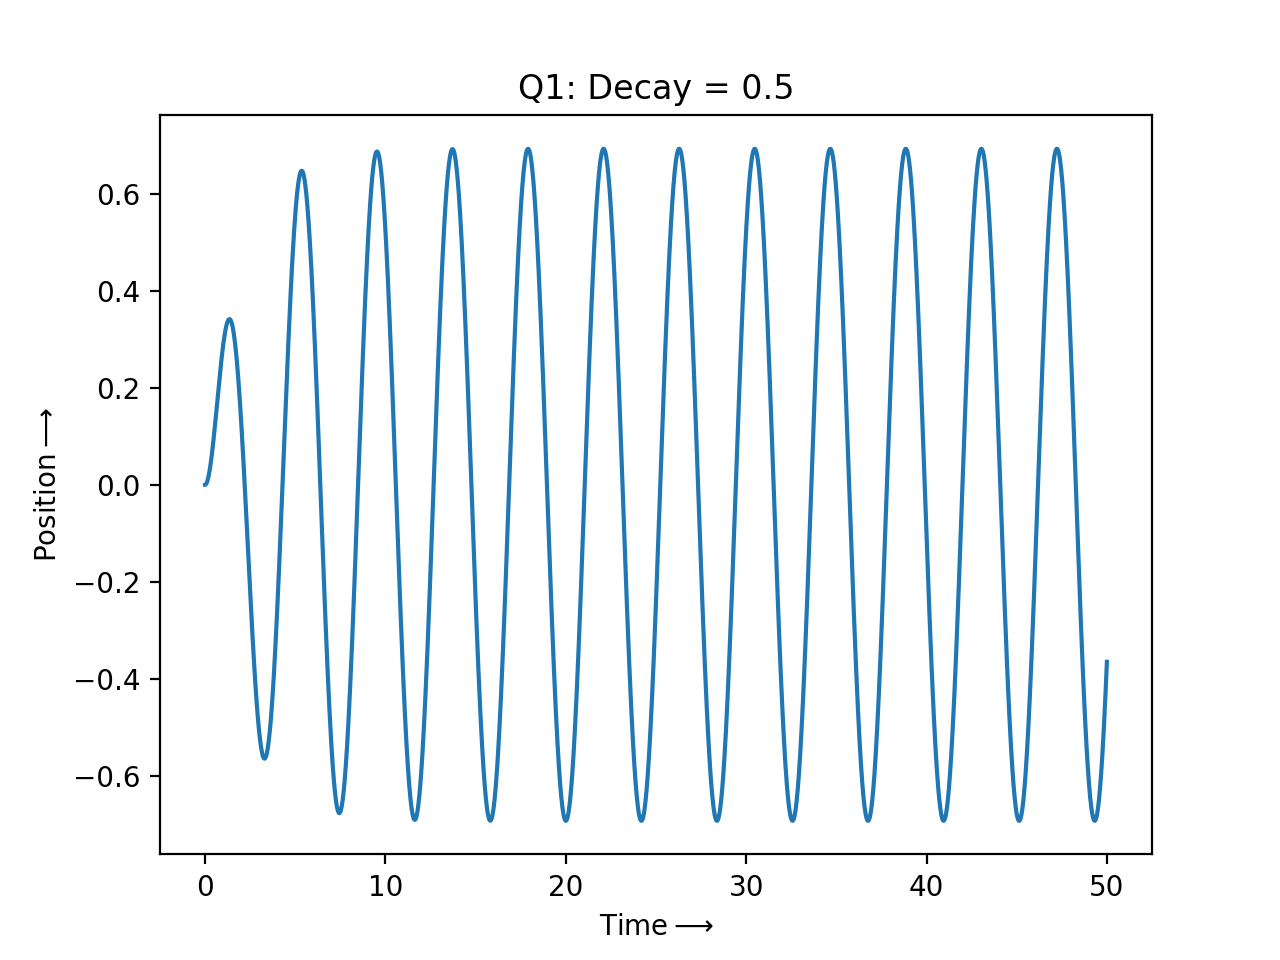
\includegraphics[scale=0.6]{Q1_1.png}
\caption{System Response with Decay = 0.5}
\label{fig:System Response with Decay = 0.5}
\end{figure}
\newpage

\begin{figure}[tbh!]
\centering
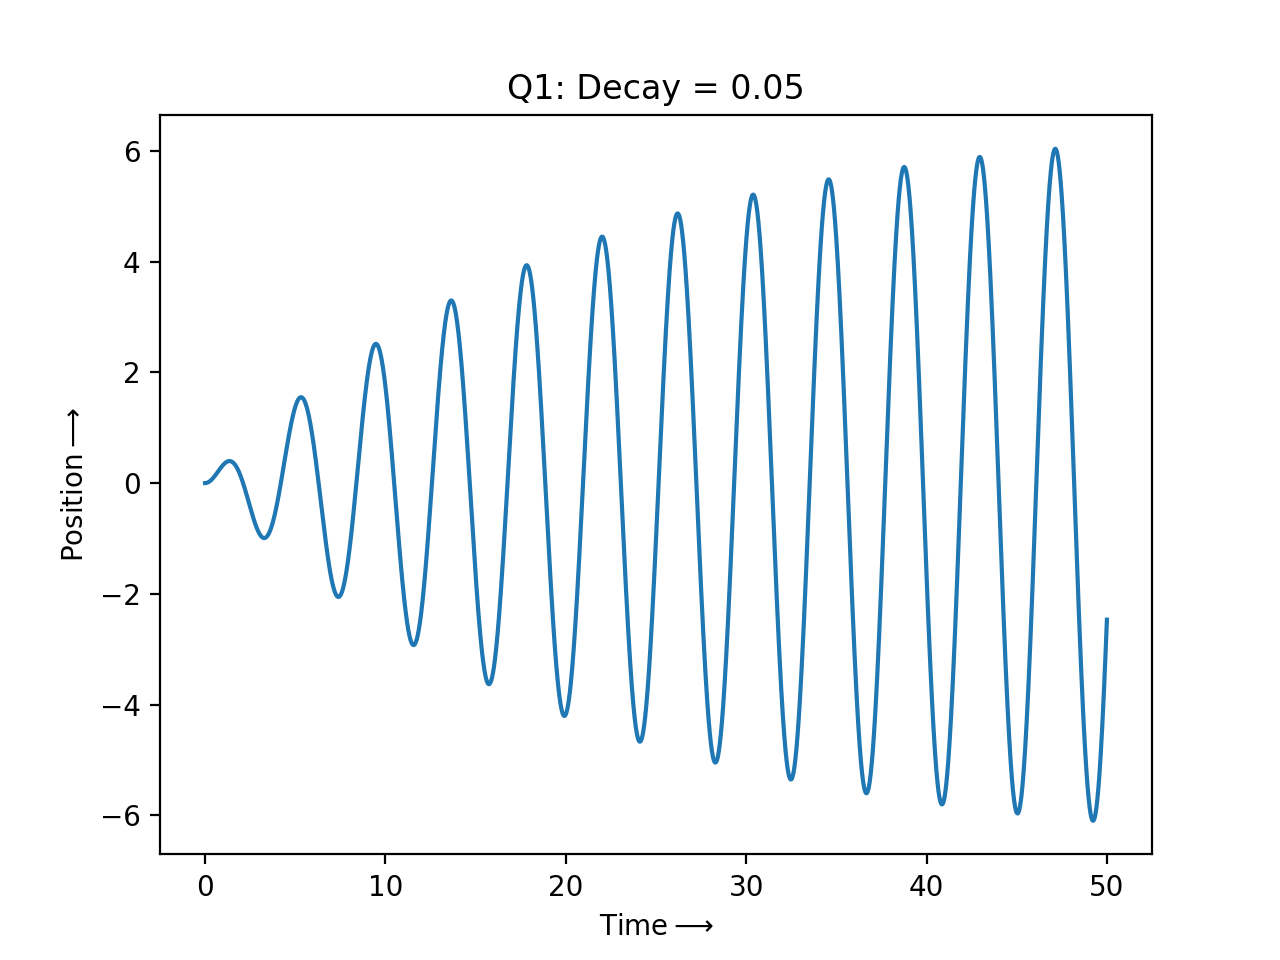
\includegraphics[scale=0.6]{Q1_2.png}
\caption{System Response with Decay = 0.05}
\label{fig:System Response with Decay = 0.05}
\end{figure}

For different values of decay constant, system gives similar final output except the time taken to reach steady state changes.

\section{Question 3}
We now simulate the above equation but with varying frequencies this time.

\begin{lstlisting}
#Q3
def Q_3():
	#Helper function which returns input function values at given time stamps
	def input_time(freq,decay_constant,time):
		cos = np.cos(freq*time)
		exp = np.multiply(np.exp(-decay_constant*time),np.heaviside(time,0.5))
		return np.multiply(cos,exp)

	#Looping through different values of frequency and plotting the output time domain simulation
	for freq in np.arange(1.4,1.6,0.05):
		transfer_function = sp.lti([1],[1,0,2.25])
		time_stamps = np.linspace(0,100,1000)

		#Simulating
		_,response,_ = sp.lsim(transfer_function,input_time(freq,0.05,time_stamps),time_stamps)
		g1 = General_Plotter("Time$\longrightarrow$","Position$\longrightarrow$","Q3: Frequency = %s"%freq,[])
		g1.line_plot(time_stamps,response)

Q_3()
\end{lstlisting}
The results are the following,
\begin{figure}[tbh!]
\centering
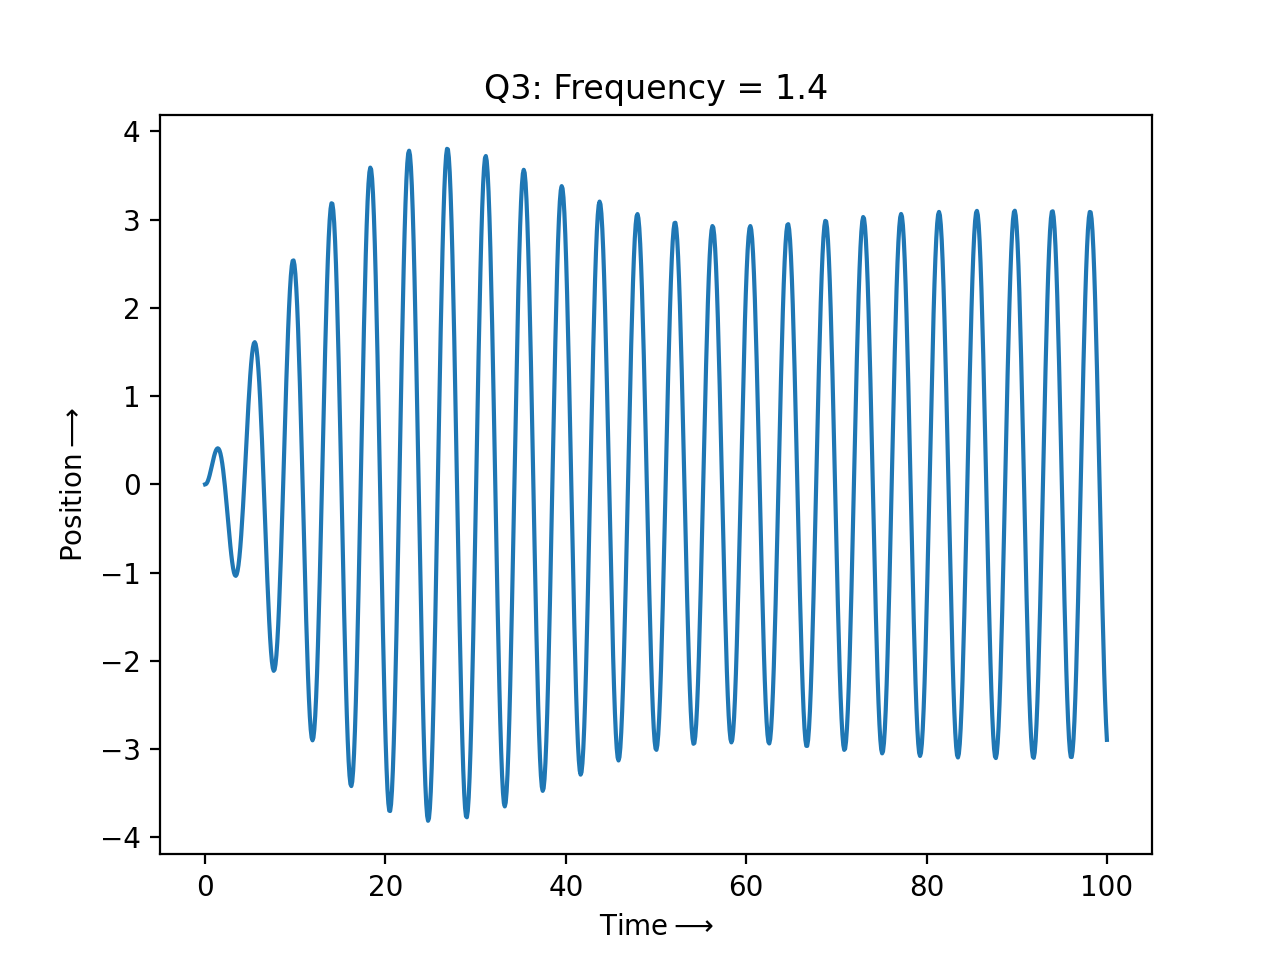
\includegraphics[scale=0.6]{Q3_1.png}
\caption{System Response with frequency = 1.4}
\label{fig:System Response with frequency = 1.4}
\end{figure}

\begin{figure}[tbh!]
\centering
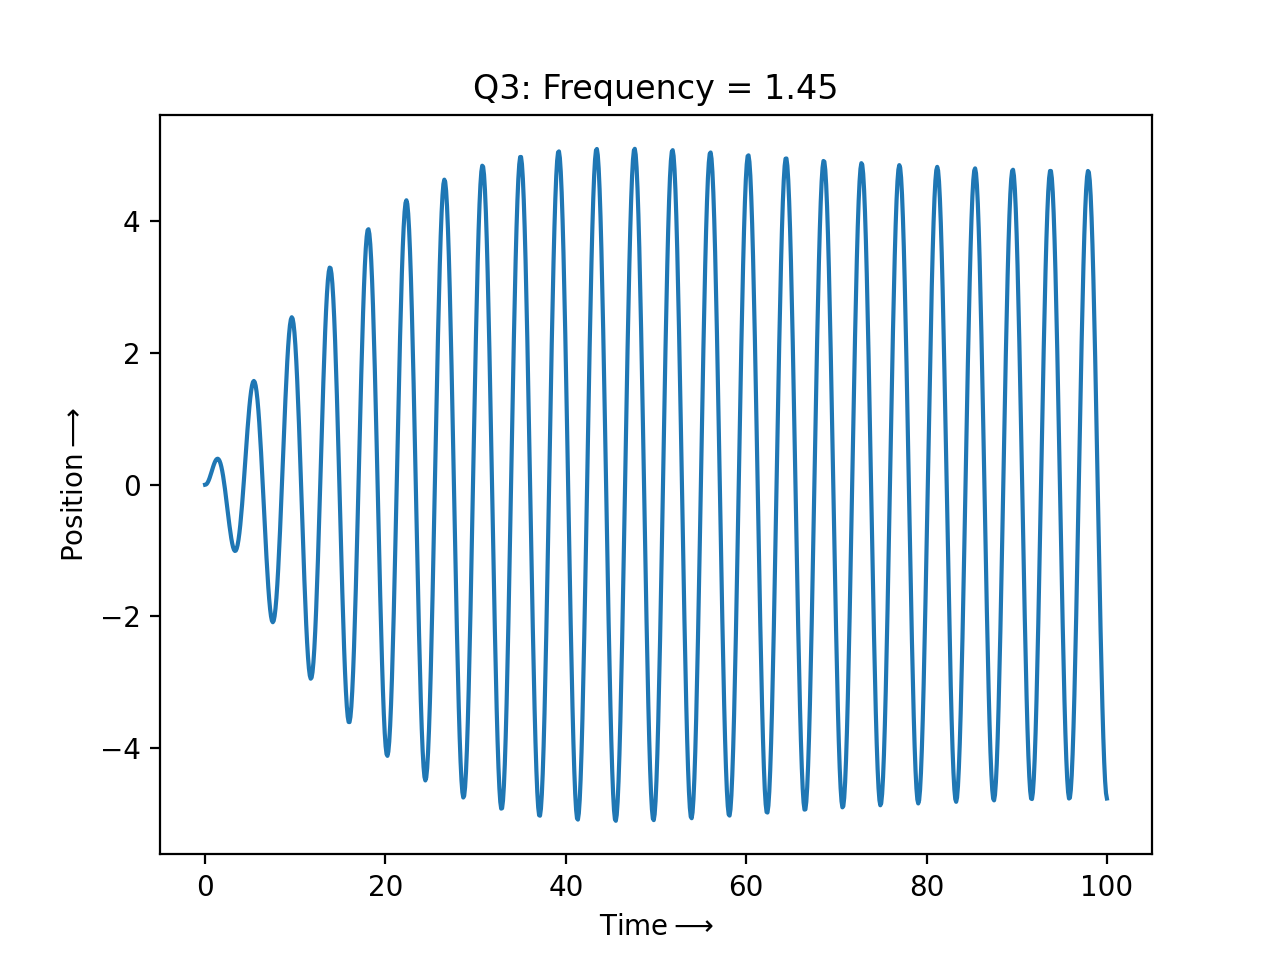
\includegraphics[scale=0.6]{Q3_2.png}
\caption{System Response with frequency = 1.45}
\label{fig:System Response with frequency = 1.45}
\end{figure}

\begin{figure}[tbh!]
\centering
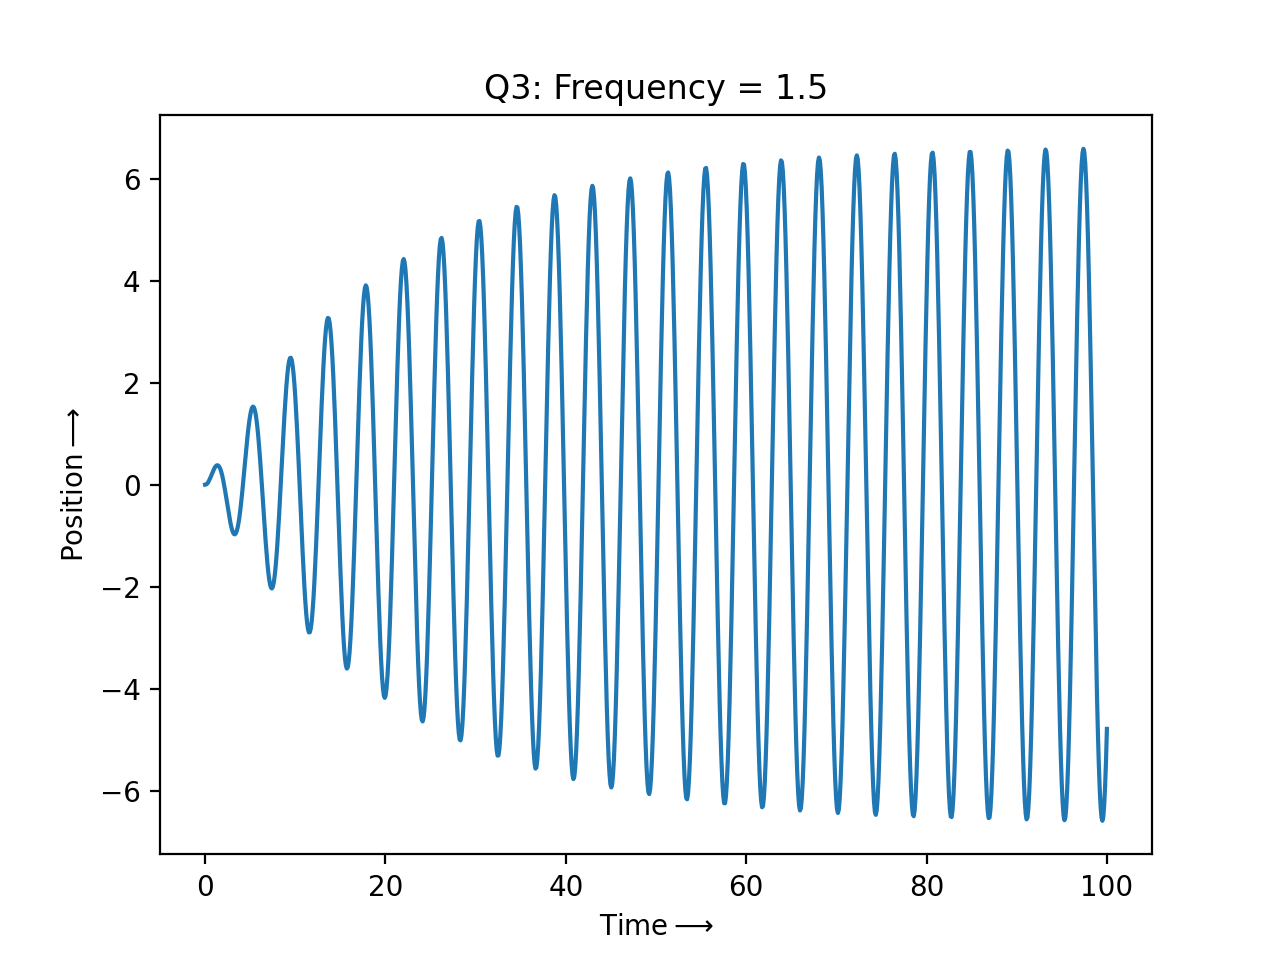
\includegraphics[scale=0.6]{Q3_3.png}
\caption{System Response with frequency = 1.5}
\label{fig:System Response with frequency = 1.5}
\end{figure}

\begin{figure}[tbh!]
\centering
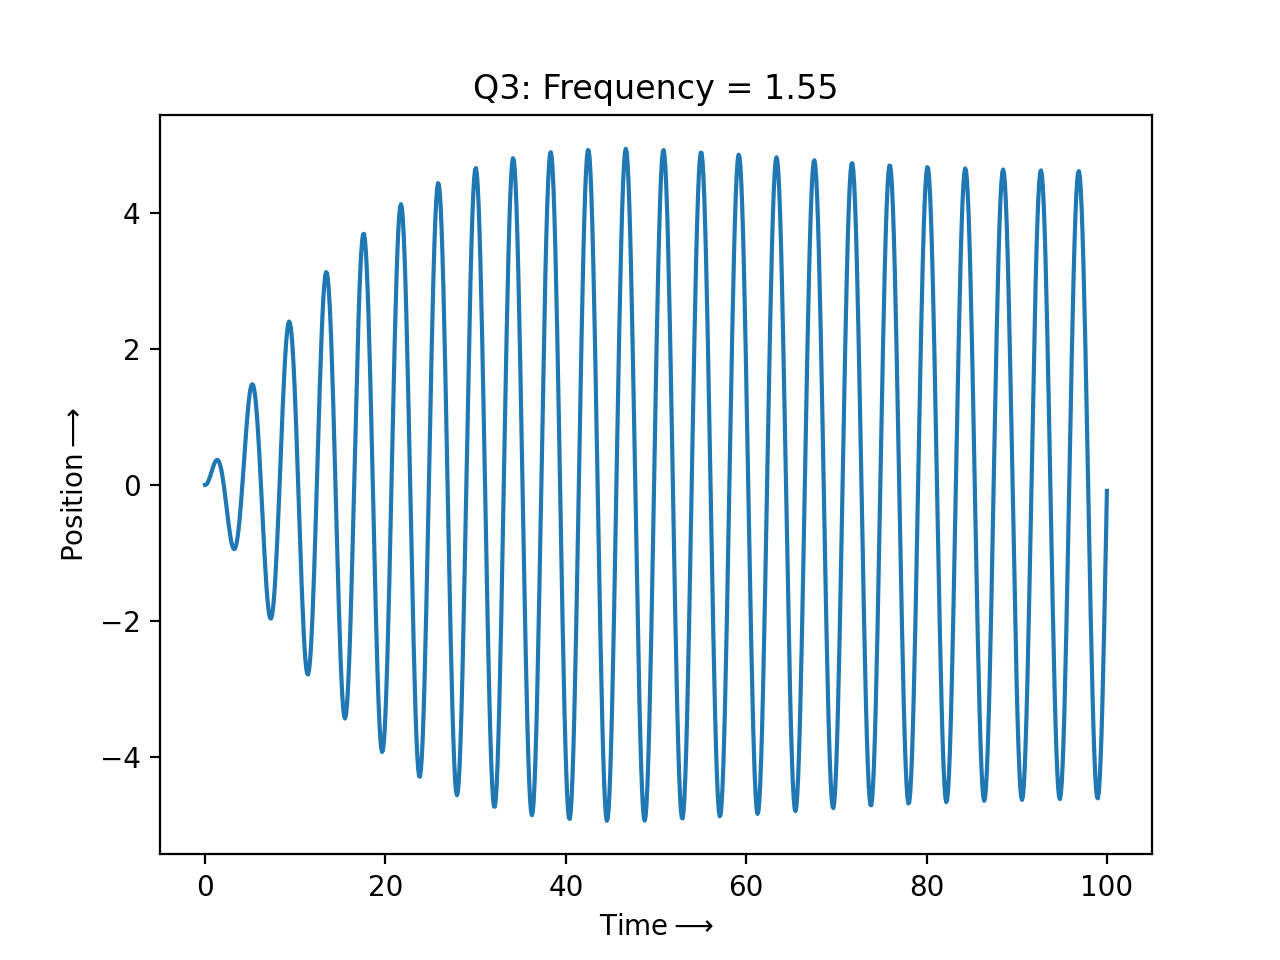
\includegraphics[scale=0.6]{Q3_4.png}
\caption{System Response with frequency = 1.55}
\label{fig:System Response with frequency = 1.55}
\end{figure}
\clearpage

\begin{figure}[tbh!]
\centering
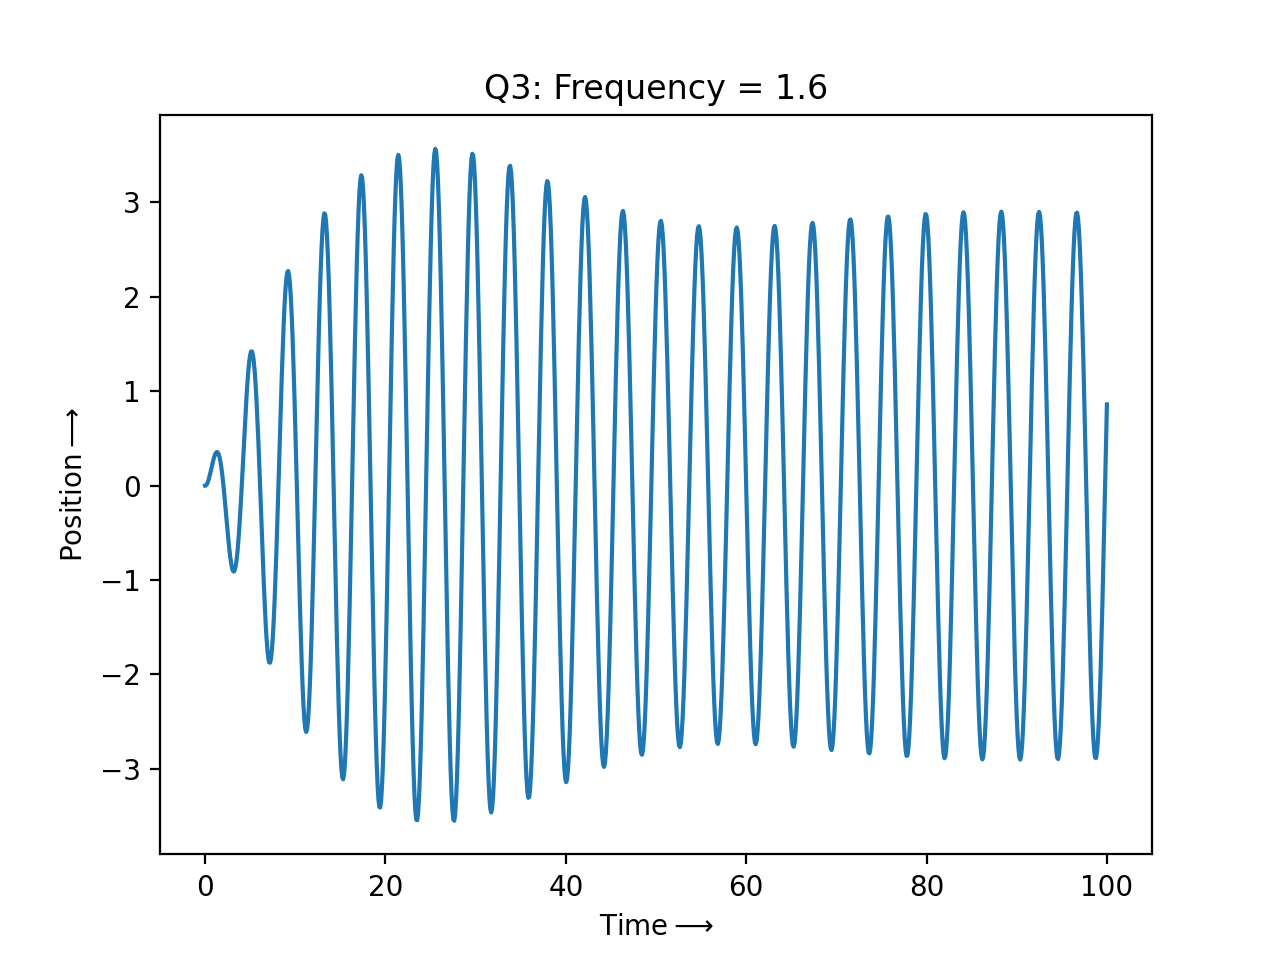
\includegraphics[scale=0.6]{Q3_5.png}
\caption{System Response with frequency = 1.6}
\label{fig:System Response with frequency = 1.6}
\end{figure}
We notice that the value of amplitude is maximum for frequency = 1.5, which is true because it is also the natural frequency of our system.

\section{Question 4}
We now consider a coupled Differential system
\begin{equation}
    \ddot x + (x-y) = 0
\end{equation}
and 
\begin{equation}
    \ddot y + 2(y-x) = 0
\end{equation}

with the initial conditions: $\dot x(0) =0,\dot y(0) =0,x(0) =1,y(0) =0$.
Taking Laplace Transform and solving for $X(s)$ and $Y(s)$, We get:
\begin{equation}
    X(s) = \frac{s^2+2}{s^3 + 3s}
\end{equation}
\begin{equation}
    Y(s) = \frac{2}{s^3 + 3s}
\end{equation}
Thus in laplace domain both equations are uncoupled. We find the corresponding equations in time domain

\begin{lstlisting}
#Q4
def Q_4():
	#Laplace function for x and y obtained by decopling the equations
	laplace_function_x = sp.lti(np.poly1d([1,0,2]),np.poly1d([1,0,3,0]))
	laplace_function_y = sp.lti(np.poly1d([2]),np.poly1d([1,0,3,0]))
	time_stamps = np.linspace(0,20,1000)

	#Obtaining the output in time domain for each laplace function
	response_x = sp.impulse(laplace_function_x,None,time_stamps)
	response_y = sp.impulse(laplace_function_y,None,time_stamps)

	g1 = General_Plotter("Time$\longrightarrow$","X$\longrightarrow$","Q4: X vs time",[])
	g1.line_plot(response_x[0],response_x[1])

	g1 = General_Plotter("Time$\longrightarrow$","Y$\longrightarrow$","Q4: Y vs time",[])
	g1.line_plot(response_y[0],response_y[1])

Q_4()
\end{lstlisting}
The corresponding graphs are,
\begin{figure}[h!]
\centering
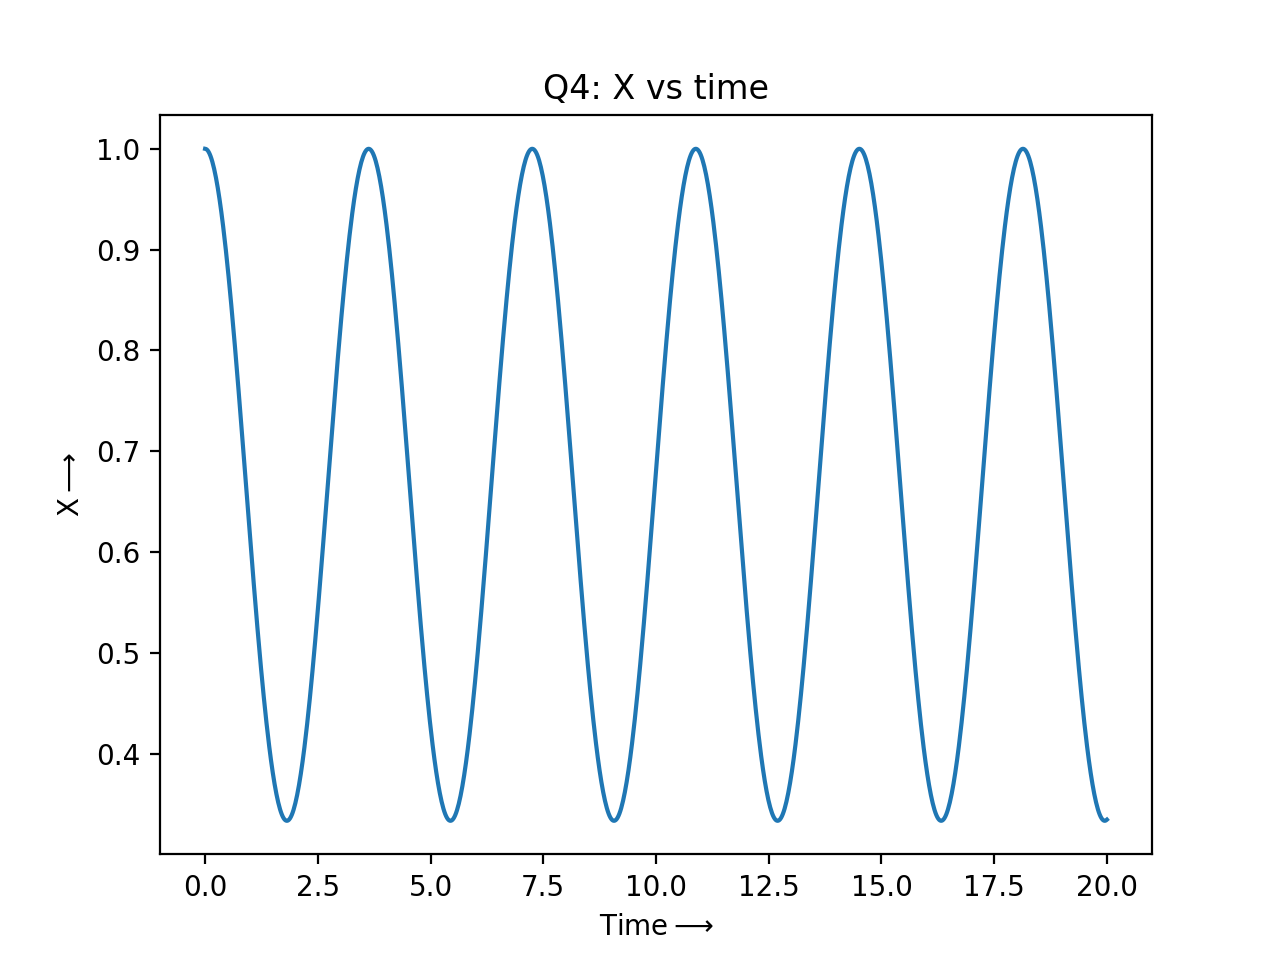
\includegraphics[scale=0.6]{Q4_1.png}
\caption{Value of X vs Time}
\label{Value of X vs Time}
\end{figure}
\clearpage

\begin{figure}[h!]
\centering
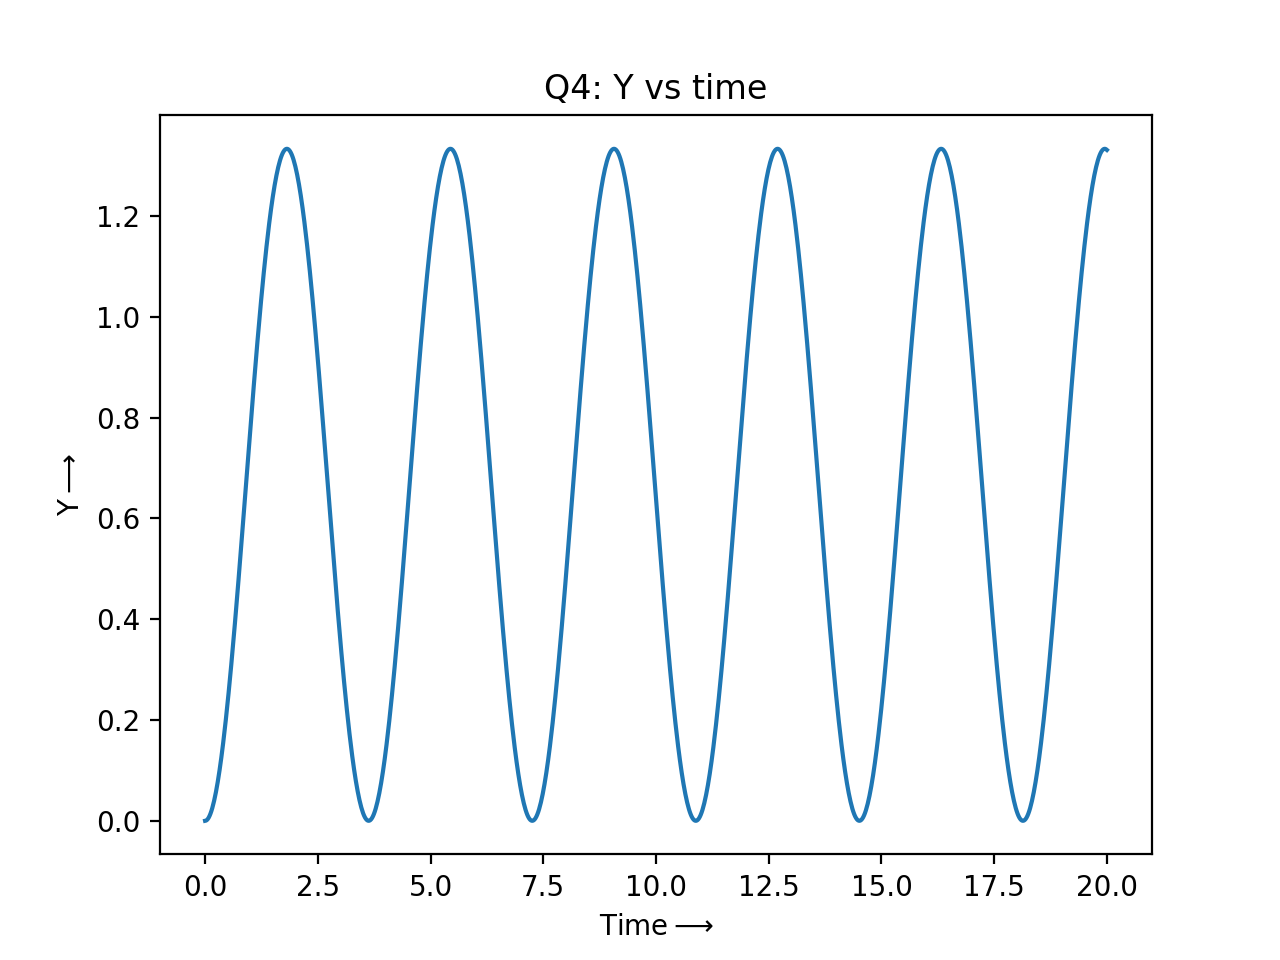
\includegraphics[scale=0.6]{Q4_2.png}
\caption{Value of Y vs Time}
\label{Value of Y vs Time}
\end{figure}

We notice that the outputs of this system are 2 sinusoids which are $90\degree$ out of phase. This system can be realized physically by creating an undamped single spring double mass system where x and y are position values of the blocks.

\section{Question 5}
Here, we plot the bode plot of the transfer function of the low-pass filter circuit given in the question.
\begin{equation}
    H(s) = \frac{1}{LCs^2 + RCs + 1}
\end{equation}

\begin{lstlisting}
#Q5
def Q_5():
	#Transfer function for the system
	transfer_function = sp.lti(np.poly1d([1000000]),np.poly1d([0.000001,100,1000000]))

	#Obtaining and plotting the bode plot of the transfer function
	freq,magnitude,phase = transfer_function.bode()

	plt.subplot(2,1,1)
	plt.semilogx(freq,magnitude)
	plt.ylabel(r'$|H(s)|$')
	plt.subplot(2,1,2)
	plt.semilogx(freq,phase)
	plt.ylabel(r'$\angle(H(s))$')
	plt.suptitle("Q5: Bode plot of two port network")
	plt.show()
	return transfer_function

transfer_function = Q_5()
\end{lstlisting}

\begin{figure}[h!]
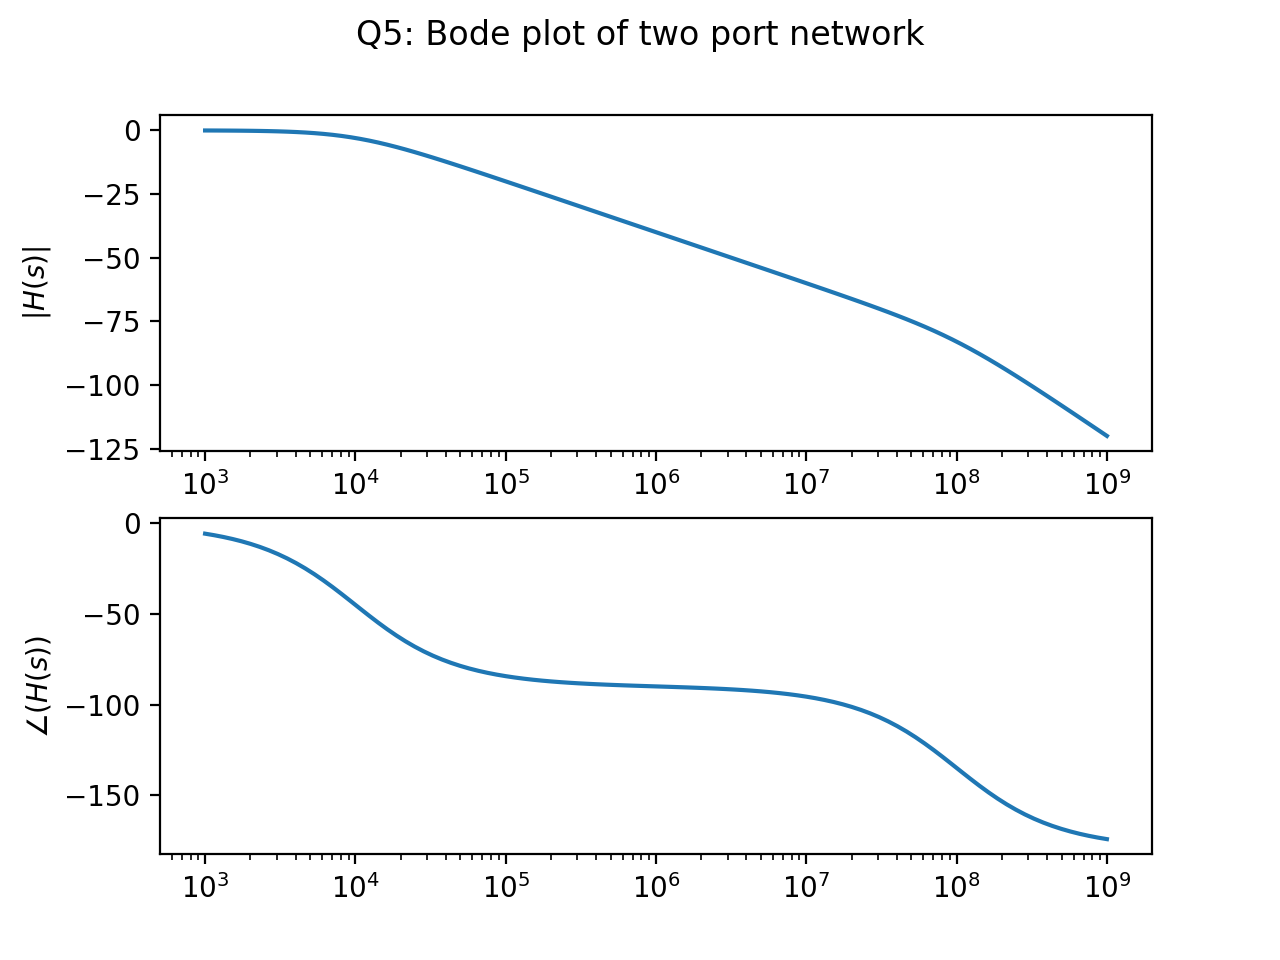
\includegraphics[scale=0.6]{Q5.png}
\centering
\caption{Bode Plots For RLC Low pass filter}
\label{fig:Bode Plots For RLC Low pass filter}
\end{figure}

\section{Question 6}
Now we find output voltage for a given input voltage $V_i(t)$,
\begin{equation}
V_i(t) = (cos(10^3t) - cos(10^6t))u(t)
\end{equation}
We plot them for two time ranges i.e. for $0<t<30\mu s$ and $0<t<10ms$

\begin{lstlisting}
#Q6
def Q_6(transfer_function):
	#Simulating and plotting Q5 for given input for time uptill 30us 
	time = np.linspace(0,30*0.000001,1000)
	vi = np.multiply(np.cos(1000*time)-np.cos(1000000*time),np.heaviside(time,0.5))
	_,output_time,_ = sp.lsim(transfer_function,vi,time)
	g1 = General_Plotter("Time$\longrightarrow$","Voltage$\longrightarrow$","Q6: Voltage uptill 30$\mu$s",[])
	g1.line_plot(time,output_time)
	
	#Simulating and plotting Q5 for given input for time uptill 1ms
	time = np.linspace(0,10*0.001,100000)
	vi = np.multiply(np.cos(1000*time)-np.cos(1000000*time),np.heaviside(time,0.5))
	_,output_time,_ = sp.lsim(transfer_function,vi,time)
	g1 = General_Plotter("Time$\longrightarrow$","Voltage$\longrightarrow$","Q6: Voltage uptill 10ms",[])
	g1.line_plot(time,output_time)

Q_6(transfer_function)
\end{lstlisting}

\begin{figure}[tbh!]
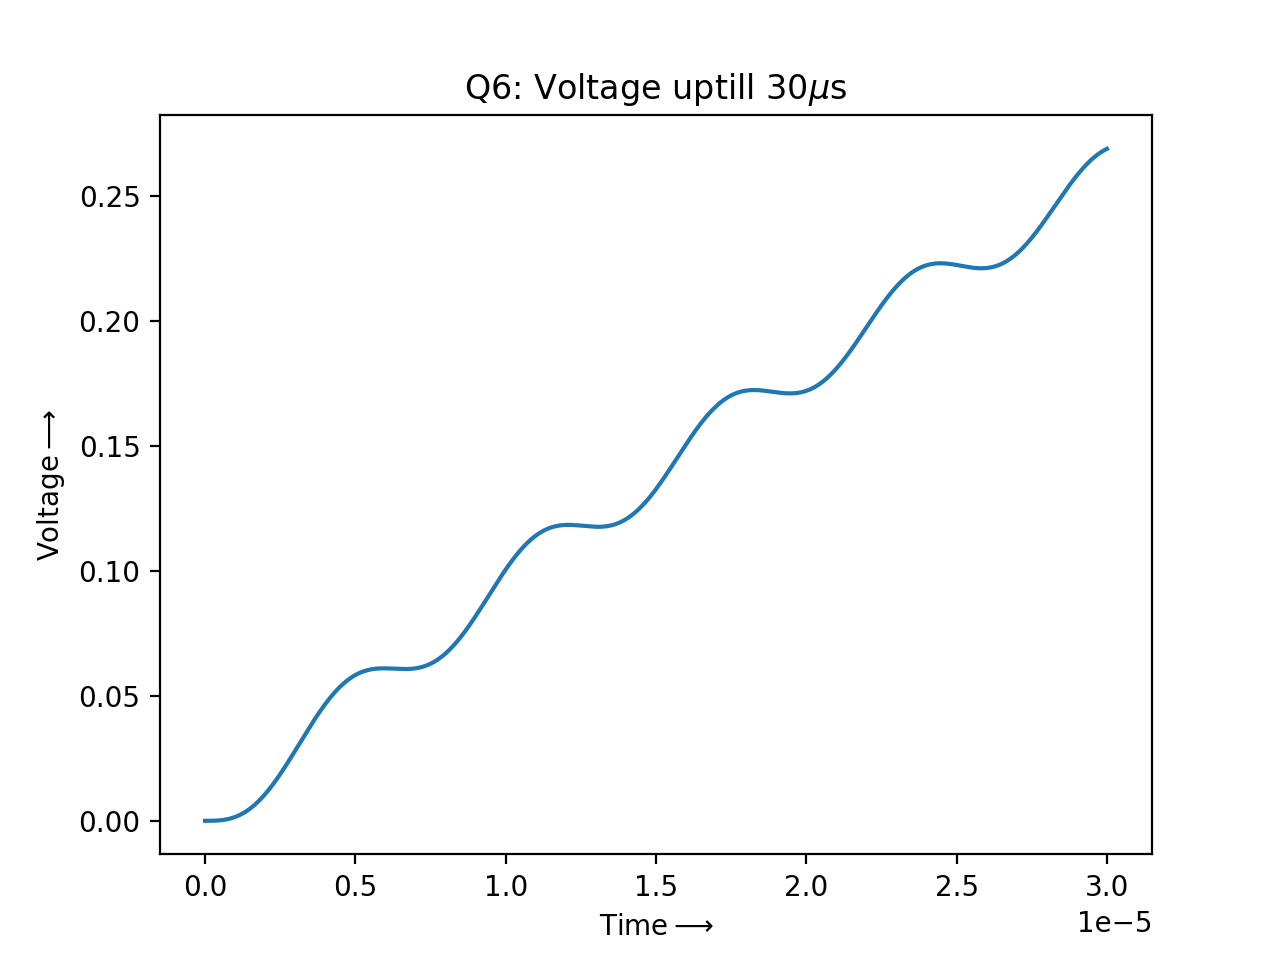
\includegraphics[scale=0.6]{Q6_1.png}
\centering
\caption{System response for t$<$30us}
\label{fig:System response for t<30us}
\end{figure}
\clearpage
\begin{figure}[tbh!]
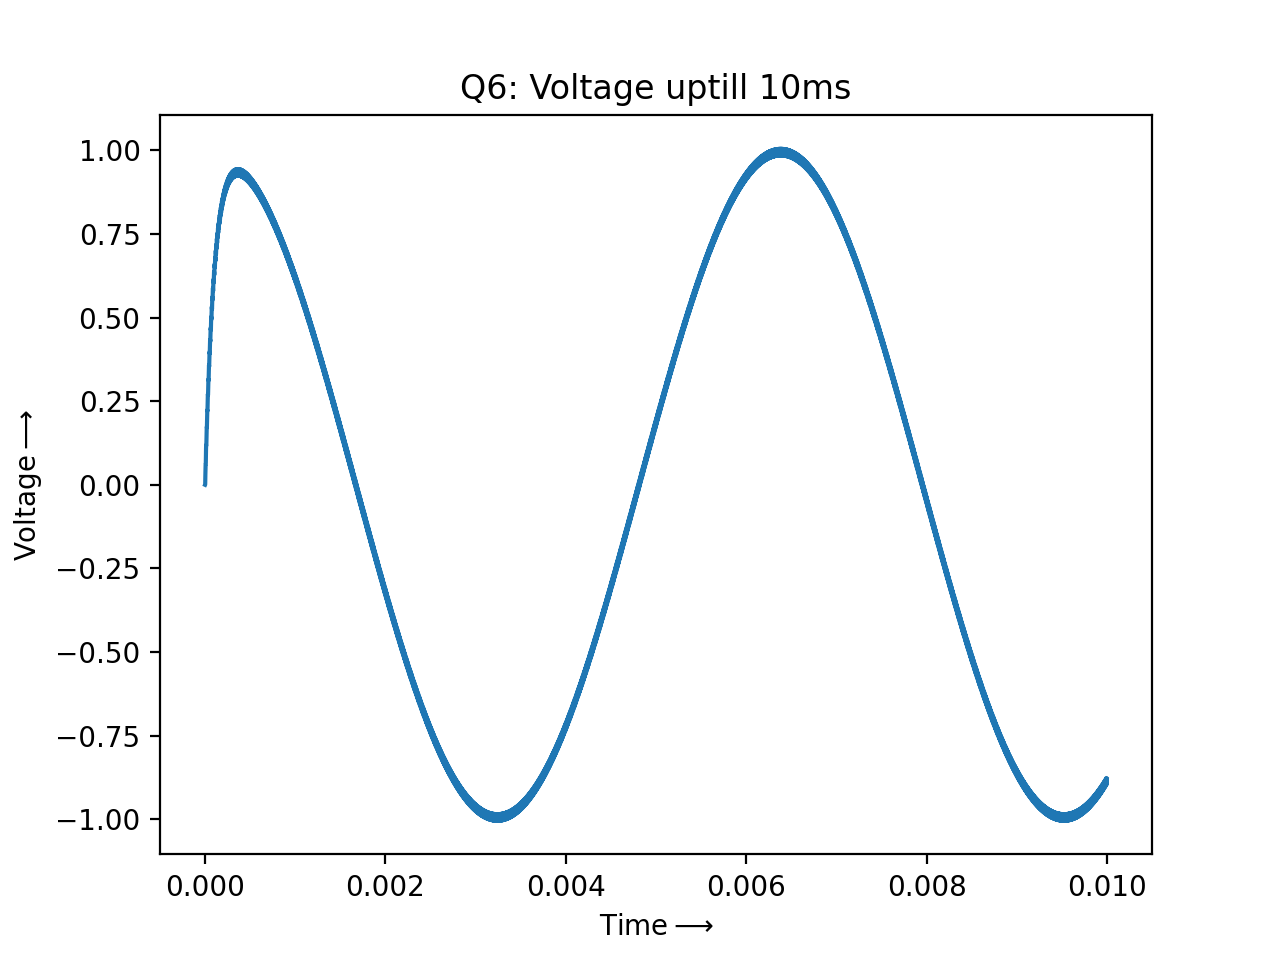
\includegraphics[scale=0.6]{Q6_2.png}
\centering
\caption{System response for t$<$10ms}
\label{fig:System response for t<10ms}
\end{figure}
The oscillations in the curve in small time range such as for the $30\mu s$ curve are due to the high frequency component of the input.

However as, the system is low-pass filter, it will allow low frequencies as $10^3$ to pass, however frequencies such as $10^6$ will get damped.

We can see that amplitude of high frequencies have dropped to almost 0.02 on zooming.
\begin{figure}[tbh!]
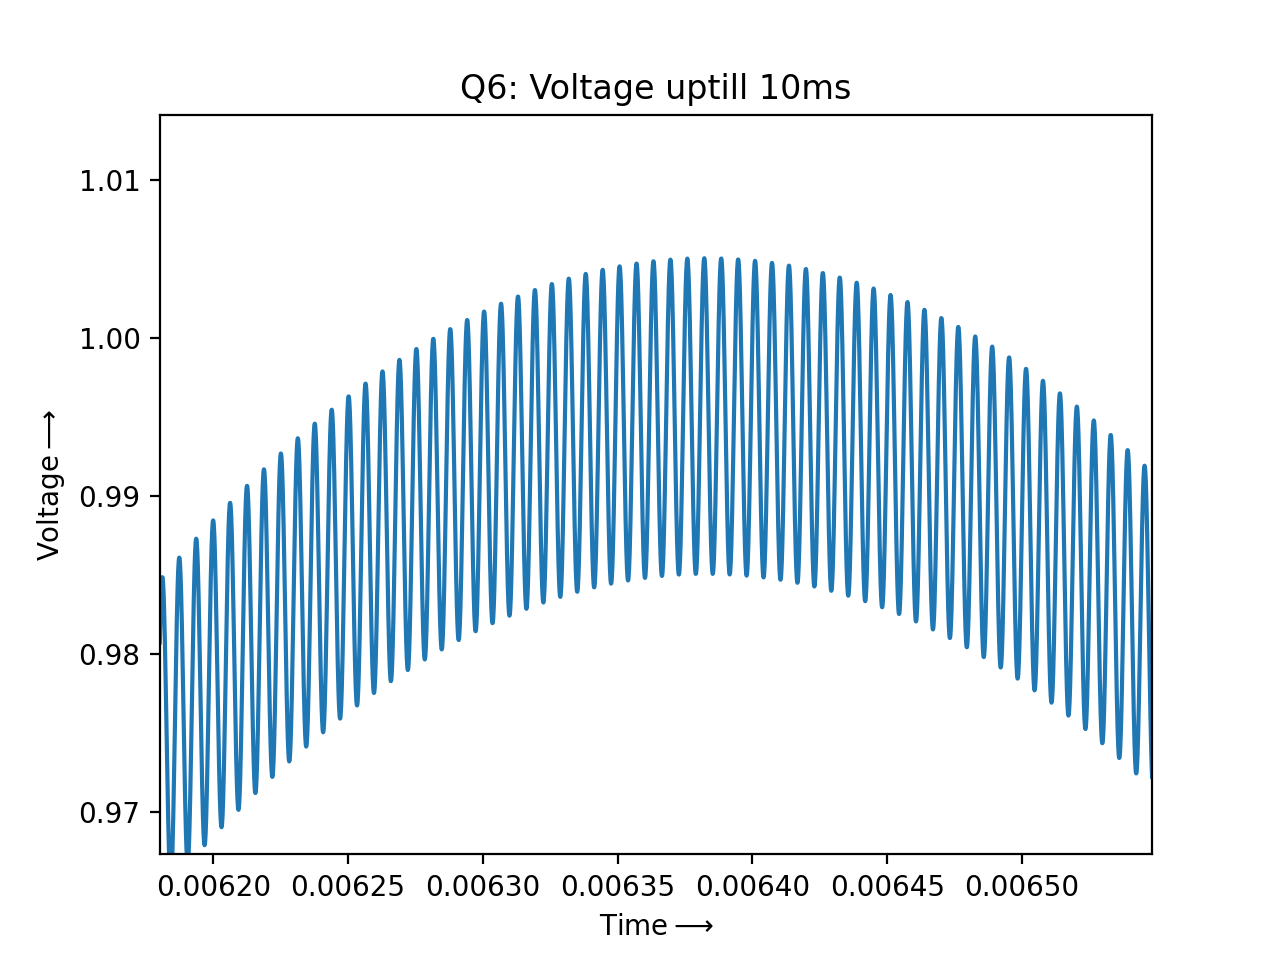
\includegraphics[scale=0.6]{Q6_3.png}
\centering
\caption{Zoomed System response for t$<$10us}
\label{fig:Zoomed System response for t<10us}
\end{figure}

\section{Conclusion}
We used the scipy.signal library to solve circuits and equations in laplace domain including forced response of simple spring body system, a coupled spring problem and a low-pass filter circuit was analysed and output signal found for a mixed frequency input signal.

\end{document}
